En el siguiente capítulo se desarollan las herramientas de gestión lean utilizadas en el proyecto además de exponer una breve explicación de la metodología y su implantación en los últimos años.

\section{Definición de la metodología lean}

La gestión Lean es un concepto moderno para la optimización de procesos en toda la cadena de valor \cite{helmold_progress_2019}.
Se centra en hacer que las ineficiencias, o desperdicios, sean transparentes y en alterarlas para convertirlas en actividades que añadan valor \cite{helmold_global_2016}.
La cadena de valor abarca en este contexto desde los proveedores, pasando por las propias operaciones, hasta los clientes \cite{slack_operations_2010}.
Las ineficiencias son todo aquello, por ejemplo, una actividad, un proceso y un producto, que se considera algo por lo que los clientes no están dispuestos a pagar o a gastar medios financieros.

El cliente es el punto central del concepto lean.
Los principales objetivos de la filosofía lean son crear valor para el cliente mediante la optimización de los recursos y crear un flujo de trabajo constante basado en las demandas reales de los clientes \cite{ohno_toyota_1988}. Busca eliminar cualquier pérdida de tiempo, esfuerzo o dinero identificando cada paso en un proceso de negocio y luego revisando o recortando los pasos que no crean valor \cite{bertagnolli_lean_2018}.

La filosofía tiene sus raíces en Japón y las operaciones, pero actualmente está ampliamente extendida por todo el mundo y las industrias.
Sus puntos centrales son los siguientes:

\begin{itemize}
    \item Poner al cliente en el centro de la operación.
    \item Definir el valor y el valor añadido desde el punto de vista del cliente final.
    \item Eliminar todos los residuos en todos los ámbitos de la cadena de valor.
    \item Mejorar continuamente todas las actividades, procesos, objetivos y personas.
    \item Situar a las personas en el centro de los servicios y procesos de valor añadido.
\end{itemize}

La gestión lean facilita el liderazgo y la responsabilidad compartida mientras que la mejora continua garantiza que cada empleado contribuya al proceso de mejora.
La metodología actúa como guía para construir una organización sólida y de éxito que progresa constantemente, identificando los problemas reales y resolviéndolos.
Lean se basa en el sistema de producción Toyota, creado a finales de los años cuarenta.
Toyota puso en práctica los cinco principios de la gestión ajustada con el objetivo de reducir la cantidad de procesos que no producían valor, lo que se conoce como \textit{Toyota Way}.

Al aplicar los cinco principios, se encontraton mejoras significativas en eficiencia, productividad, rentabilidad y duración de los ciclos.
Lean incorpora cinco principios rectores que son utilizados por los directivos de una organización como directrices de la metodología \cite{helmold_progress_2019}. Los cinco principios son:

\begin{itemize}
    \item Identificar el valor en todos los procesos de la cadena de valor.
    \item Realización de mapas de flujo de valor.
    \item Crear un flujo de trabajo continuo.
    \item Establecer un sistema \textit{pull} en el que los clientes sean el centro de atención.
\end{itemize}

Identificar el valor, el primer paso en la gestión lean, significa encontrar el problema que el cliente necesita resolver y convertir el producto en la solución.
En concreto, el producto debe ser la parte de la solución por la que el cliente esté dispuesto a pagar.
Cualquier proceso o actividad que no añada valor, es decir, que no aporte utilidad y el cliente no está dispuesto a pagar por ello, importancia o valor al producto fnal se considera residuo y debe eliminarse \cite{liker_toyota_2006}.

\textit{Value Stream Mapping} se refiere a la herramienta que se utiliza para mapear el flujo de trabajo de la empresa, incluyendo todas las acciones y personas que contribuyen al proceso de creación y entrega del producto final al consumidor.
Trazar la cadena de valor ayuda a los directivos a visualizar qué procesos están dirigidos por qué equipos y a identificar a las personas responsables de medir, evaluar y mejorar el proceso.
La visualización ayuda a los directivos a determinar qué partes del sistema no aportan valor al flujo de trabajo \cite{slack_operations_2010}.

Crear un flujo de trabajo continuo significa garantizar que el flujo de trabajo de cada equipo progrese sin problemas y evitar las interrupciones o cuellos de botella que pueden producirse con el trabajo en equipos interfuncionales.
\textit{Kanban}, una técnica de gestión ajustada que utiliza una señal visual para desencadenar la acción, se utiliza para facilitar la comunicación entre equipos para que puedan abordar lo que hay que hacer y cuándo hay que hacerlo.
En el proceso de trabajo total en una colección de partes más pequeñas y visualizar el flujo de trabajo en este sentido facilitan la eliminación factible de interrupciones y interrupciones y bloqueos.

Desarrollar un sistema \textit{pull} asegura que el flujo de trabajo continuo se mantenga estable y garantiza que los equipos entreguen las asignaciones de trabajo más rápido y con menos esfuerzo. Un sistema pull es una técnica lean específica que reduce los residuos de cualquier producción. Garantiza que sólo se inicie un nuevo trabajo si hay demanda del mismo, lo que ofrece la ventaja de minimizar los gastos generales y optimizar los costes de almacenamiento.

El último principio es la mejora continua y puede considerarse el paso más importante del método de gestión ajustada.
Facilitar la mejora continua se refiere a una serie de técnicas que se utilizan para identificar lo que una organización ha hecho, lo que necesita hacer, los posibles obstáculos que puedan surgir y cómo todos los miembros de la organización pueden mejorar sus procesos de trabajo.
El sistema lean no está aislado ni es inmutable, por lo que pueden surgir problemas en cualquiera de los otros cuatro pasos.
Asegurarse de que todos los empleados contribuyen a la mejora continua del flujo de trabajo protege a la organización cuando surgen problemas.
La dirección debe crear un entorno y una cultura en los que todos los empleados puedan trabajar de acuerdo con los cinco principios \cite{ohno_toyota_1988,bertagnolli_lean_2018}.

\section{La gestión lean en el sector sanitario}

Lean parte del rechazo al despilfarro. Atribuido a Taiichi Ohno, el sistema Lean se desarrolló en los años 50 y 60 para ofrecer la mejor calidad, el menor coste y el menor plazo de entrega mediante la eliminación de los residuos.
El término japonés para lo que las empresas estadounidenses suelen clasificar como despilfarro es \textit{muda} y fue definido por Fujio Cho de Toyota como "cualquier cosa que no sea la cantidad mínima de equipo, espacio y tiempo del trabajador, que son absolutamente esenciales para añadir valor al producto" \cite{helmold_lean_2020}.

La presencia de este tipo de residuos en un sistema repercute negativamente en el plazo de entrega, el coste y la calidad.
A principios de los años 80, empresas de otros sectores, como el sanitario, comprendieron que la introducción de los principios lean conllevaría varias ventajas.
El despilfarro en la sanidad puede describirse, entre otros elementos, en el transporte excesivo de medicamentos o pacientes, el tiempo de espera para los tratamientos o la infrautilización de equipos y máquinas en los hospitales. Además, las duplicaciones e ineficiencias del personal de enfermería también pueden repercutir en la creación de residuos.

Aunque la metodología de mejora empresarial lean se desarrolló inicialmente para mejorar la calidad y la productividad de las fábricas de automóviles, se ha utilizado con gran éxito en industrias y entornos de todo tipo, como el desarrollo de software, la administración pública, el comercio minorista y otros entornos de servicios.
Las organizaciones sanitarias, en particular, han descubierto que el enfoque puede utilizarse para reducir costes y mejorar la calidad y la satisfacción de los pacientes al mismo tiempo \cite{millard_how_nodate}.
Uno de los principios básicos del lean es la eliminación del despilfarro, que se define como todo aquello que no añade valor al cliente.
Los profesionales se centran en ocho tipos específicos de residuos.
Son tan comunes en la sanidad como en la industria.
Por lo tanto, la gestión ajustada tiene como objetivo eliminar, por ejemplo, los tiempos de espera o el exceso de medicación como se muestra en la Tabla~\ref{tab:timwood}.

\begin{table}
    \centering
    \begin{tabular}{llp{10cm}}
        \toprule
        Letra & Despilfarro     & Definición                                                                         \\
        \midrule
        T     & Transport       & Movimiento excesivo de personas, información o materiales                          \\
        I     & Inventory       & Stock excesivo y retraso en la información o productos                             \\
        M     & Motion          & Cualquier movimiento que no añada valor al producto o al proceso                   \\
        W     & Waiting         & Largos periodos de inactividad de personas, información, maquinaria o   materiales \\
        O     & Overutilization & Producir más o antes de que lo requiera el cliente                                 \\
        O     & Overmedication  & Utilización de las herramientas, procedimientos o sistemas incorrectos             \\
        D     & Defects         & Errores frecuentes en los trámites o en la calidad del producto                    \\
        \bottomrule
    \end{tabular}
    \caption{TIMWOOD, el acrónimo que define los siete despilfarros en el sector sanitario}
    \label{tab:timwood}
\end{table}

\subsection{Transporte}

El despilfarro del transporte se produce cuando los materiales se trasladan de un lugar a otro de forma ineficaz. En sanidad se produce cuando:

\begin{itemize}
    \item Los pacientes son trasladados de un departamento a otro o de una habitación a otra
    \item Los medicamentos se trasladan de la farmacia al lugar donde se necesitan
    \item Los suministros se trasladan del almacén a la planta
\end{itemize}

Algunos de estos transportes se consideran residuos "necesarios" que hay que minimizar aunque no puedan eliminarse por completo.

\subsection{Inventario}

Los fabricantes han adoptado en gran medida un enfoque de inventario justo a tiempo para reducir los costes relacionados con el almacenamiento, el movimiento, el deterioro y el desperdicio.
Las organizaciones sanitarias buscan hacer lo mismo en lo que se refiere a:

\begin{itemize}
    \item Medicación que esté cerca de la fecha de caducidad
    \item Exceso de consumibles
    \item Formularios preimpresos
    \item Exceso de material de cabecera
\end{itemize}

\subsection{Movimiento}

El movimiento se refiere al desplazamiento innecesario de personas dentro de una instalación.
Este ocurre cuando:

\begin{itemize}
    \item La distribución de las oficinas o del hospital no es coherente con el flujo de trabajo.
    \item Los suministros no se almacenan donde se necesitan
    \item Los equipos no están bien situados
\end{itemize}

El primer paso para combatir los despilfarros del lean es reconocerlos dentro de su organización.
En la mayoría de los casos, el examen de cada uno de estos factores específicos que contribuyen con frecuencia al despilfarro conduce al descubrimiento de múltiples oportunidades de mejora.
También podemos esforzarnos por eliminar el despilfarro (incluidos los clics del ordenador) en los sistemas de software.

\subsection{Esperas}

En la fabricación, la espera se produce cuando las piezas no pueden salir o cuando los miembros del equipo no pueden realizar sus tareas debido a problemas, como la falta de existencias o fallos en los equipos.
La espera en la atención sanitaria es un problema tanto para los pacientes como para los proveedores.

\begin{itemize}
    \item Pacientes en salas de espera (o de examen)
    \item Funcionarios con cargas de trabajo desiguales a la espera de su próxima tarea
    \item Pacientes de urgencias y médicos a la espera de los resultados de las pruebas
    \item Pacientes de urgencias en espera de ingreso hospitalario
    \item Pacientes en espera de alta médica
\end{itemize}

\subsection{Sobreutilización}

En la industria manufacturera, la sobreproducción se traduce en un exceso de ``trabajo en curso'' o de existencias de ``productos acabados'' sin vender.
En sanidad es más difícil de detectar, pero se produce cuando los proveedores hacen más de lo que necesita el cliente en ese momento.
Incluye:

\begin{itemize}
    \item Pruebas diagnósticas innecesarias
    \item Comidas no consumidas
    \item Pedir medicamentos que el paciente no necesita
    \item Personal en horas no punta
\end{itemize}

\subsection{Sobremedicación}

Sobreprocesar significa hacer más trabajo, hacerlo más complejo o más caro de lo necesario.
Adopta la forma de:

\begin{itemize}
    \item Pedir imágenes diagnósticas complejas (resonancia magnética) cuando bastaría con un método más sencillo (radiografía)
    \item Trámites innecesarios
    \item Intervención quirúrgica en lugar de una alternativa médica igualmente eficaz
    \item Citas de seguimiento que no mejoran los resultados del paciente
    \item Tratamientos por especialistas que podrían realizar los proveedores de atención primaria
\end{itemize}

\subsection{Defectos}

Mientras que los defectos de fabricación son caros y molestos, en la atención sanitaria pueden ser mortales.
Pueden incluir:

\begin{itemize}
    \item Diagnóstico erróneo
    \item Administración de medicamentos incorrectos
    \item Afecciones adquiridas en el hospital
    \item Códigos identificativos incorrectos
\end{itemize}

El despilfarro incluye el tiempo empleado en crear un defecto, reelaborar estos defectos e inspección de estos defectos.
Aunque consideremos que la inspección es un despilfarro, no podemos hasta que no tengamos un proceso perfecto sin defectos.
Incluso Toyota aún tiene inspecciones finales cada año, pero la consideran un despilfarro que esperan eliminar algún día.

\section{Estandarización de tareas}

El trabajo estandarizado es uno de los pilares de la metodología lean, sin embargo, su aplicación en entornos alejados de la industria manufacturera, como una oficina o un hospital puede ser no tan clara.
Las dificultades de su aplicación residen principalmente en el desconocimiento de los beneficios que puede aportar, sobre todo al no ser tangibles como podría ser si se estuviera fabricando un producto.
Entre los argumentos en contra del trabajo estandarizado se encuentran \cite{locher_lean_2017}:

\begin{itemize}
    \item ``¿Por qué preocuparse de cómo llevo a cabo mis tareas siempre y cuando se termine el trabajo?''
    \item ``El trabajo estandarizado no es efectivo para las actividades creativas en oficinas y servicios''
    \item ``El entorno de oficinas es demasiado variable y no es adecuado para estandarizar''
\end{itemize}

\subsection{Propósito de la estandarización}

La estandarización de las tareas es uno de los mejores métodos para realizar una actividad de forma eficaz y eficiente. La estandarización define de la secuencia deseada de los pasos, el tiempo necesario para llevar a cabo cada uno y otros elementos que aseguren la regularidad de la actividad. De esta forma, se garantiza la realización de las tareas además de la calidad del producto, en este caso un servicio.

La documentación relacionada con la estandarización de la tarea debe ser concisa y simple.
Además debe de ser accesible para el trabajador de forma visual en su propio puesto de trabajo.
Esto no quiere decir que la documentación funcione como un manual de acogida para empleados que van a comenzar en el puesto ya que para esto existen los procedimientos operativos abiertos.
Los procedimientos, aunque funcionan para agilizar el aprendizaje del puesto, no sustituye la aplicación de la metodología de estandarización.

El nivel de detalle en el trabajo estandarizado es otro de los puntos críticos. Es necesario agrupar las tareas en los distintos procesos pero sin llegar a un nivel de detalle extremo, que aunque pueden ser útiles para el trabajador recién llegado no facilitan la compresión del proceso.

Entre los objetivos de la estandarización del trabajo se encuentra la de identificar puntos no estandarizados en los procesos para así poner en marcha la metodología. Sin embargo, esto no puede suceder si de entrada no existen estos estándares.

\begin{itemize}
    \item Incapacidad para realizar una tarea en un determinado momento
    \item Tardar más tiempo del necesario en una tarea
    \item Realizar tareas con impacto negativo en otras dependientes de esta
\end{itemize}

La rapidez con que se identifican estas situaciones es vital para devolver el proceso a su estado estandarizado.
En el plano teórico, son los propios trabajadores quienes detectan los desvío del estándar y corrigen el propio proceso hasta devolverlo a la normalidad.
Cuando esto no es posible, se hace necesario un agente externo que compruebe si los trabajadores siguen el estándar establecido.
Las actividades de observación no deben de tomarse como acciones de castigo sino como oportunidades de mejora.

Son los propios líderes quienes tienen la responsabilidad de asegurar el trabajo estandarizado en todas las áreas de la empresa. Si esto no sucede, el líder tiene la posibilidad de inferir en el proceso, por ejemplo, ofreciendo formación a los empleados con el fin de conseguir que las tareas se cumplan en tiempo y forma. Por otra parte, si se permite que el empleado realice las tareas conforme a su criterio se corre el riesgo de tener una variabilidad muy elevada. Esta variabilidad dificulta enormemente al lider corregir y valorar el trabajo de los empleados. Una de las formas de corregir la variabilidad es a través de la estandarización del trabajo.

En muchas ocasiones, se justifica la imposibilidad de aplicar la metodología lean debido a la alta variabilidad de los procesos. Sin embargo, se ignora que la aplicación de la metología trata de mitigar esta variabilidad.

\subsection{Elementos de la estandarización de tareas}

Primeramente, es necesario definir y describir las tareas que se realizan en el lugar de trabajo para, posteriormente, agruparlas y ordenarlas en una secuencia.

Igual de importante es la manera en que se realizan las distintas tareas.
Este punto es crítico ya que correponde a todo el conocimiento necesario para realizar una tarea que posee el trabajador pero que no logra transmitir adecuadamente. Documentar estos detalles es vital para conseguir una buena estandarización del proceso.
Tambien hay que tener en cuenta el nivel de detalle de la documentación.
La estandarización debe de servir al trabajador no como elemento de formación sino como referencia de qué tareas realizar y por qué.

Los punto clave a la hora de definir una tarea estandarizada deben de asegurar la correcta calidad del servicio y el cumplimiento del tiempo de realización.
En ocasiones, se da la situación de que un empleado encuentra una manera de agilizar sus operaciones y completar las tareas en menor tiempo del estimado.
Sin embargo, puede que este tipo de atajos sean perjudiciales para el empleado encargado de continuar con el trabajo ``aguas abajo'' aumentando incluso su carga de trabajo. Por esta razón, a la hora de documentar una tarea estandarizada es importante especificar el ``por qué'' de cada elemento.

Especificar la duración estimada de una tarea es importante a la hora de estandarizar un proceso.
Es posible que exista cierto recelo a la hora de incluir la duración de una tarea ya que puede dar lugar reacciones sancionadoras debido al incumplimiento de los tiempos.
Sin embargo, conocer los tiempos es vital para detectar oportunidades de mejora en el proceso por lo que es frecuente que se daten como intervalos razonables.
De esta forma, cuando una tarea sobrepase el rango previsto se identificará la tarea en la que es necesario actuar.

Asimismo, incluir en la definición de una tarea el momento concreto en el que se debe realizar ayuda a garantizar la secuencia del proceso, sobre todo cuando dependen de otros departamentos.

\subsection{Representación visual}

Visualizar la secuencia de tareas es clave a la hora de mantener el estándar ya que lo que está fuera de la vista puede estar fuera de la mente. Como una imagen vale más que mil palabras, en la Tabla~\ref{tab:ejemplo-estandar} se muestra la lista que un empleado del departamento administrativo sanitario podría realizar junto con el los plazos establecidos.
El formato de la tabla se puede modificar para adecuarse a las peculiaridades del puesto añadiendo nuevas columnas de categorías, solicitante, destino o , incluso, formularios.
De esta manera, el empleado que desempeñe el puesto sabrá en cada momento qué tareas debe realizar y si la está realizando en el tiempo adecuado.

\begin{table}
    \centering
    \begin{tabular}{p{5cm}ll}
        \toprule
        Tarea                                                             & Duración                & Frecuencia             \\
        \midrule
        Registrar las solicitudes de citas para asegurar que se completan & 5 a 10 minutos por cita & Todo el día            \\
        Generar informes para controlar la demanda                        & 5 minutos               & Viernes a las 15:00    \\
        Generar informes mensuales de utilización                         & 10 minutos              & Último viernes del mes \\
        \bottomrule
    \end{tabular}
    \caption{Ejemplo de estandarización de tareas}
    \label{tab:ejemplo-estandar}
\end{table}

\subsection{Pasos para la estandarización}

El fin de la estandarizar el trabajo no es aplicarlo a todas las actividades sino solamente a las que mayor valor aportan de cara al cliente. Es un error común que puede llegar a interpretarse negativamente como que el fin es el control total de entorno laboral. Por ello, la pregunta que se debe de hacerse el líder es : ¿en qué beneficia la estandarización de la tarea a la organización?

Las fases por las que se debe pasar a la hora de estandarizar son las siguientes:

\subsubsection{Identificar las tareas claves del puesto}

El responsable debe identificar todas las actividades que se realizan en el área.
Para ello será útil aprovechar, si los hubiera, de manuales de acogida o procedimientos antiguos antes de reunirse con los empleados.

\subsubsection{Priorizar las tareas clave por orden de importancia}

El segundo paso consiste en la ordenación de las distintas tareas según su importancia.
Como se ha mencionado anteriormente, la metodología debe aplicarse únicamente en el conjunto de tareas que aportan valor al cliente final, en un centro sanitario sería el paciente.
Además del valor, debe tenerse en cuenta el tiempo que consume la tarea al trabajador.

\subsubsection{Reunir a un grupo de personas que establezcan la estandarización}

A la hora de formar el equipo de trabajo, es importante incluir empleados que realicen las tareas descritas de forma regular.
Generalmente, no se podrá incluir en el grupo a todos los empleados, por lo que se debe de entender que se busca representar los intereses del grupo.
En los pasos posteriores, será útil que otros empleados o el líder forme parte del grupo de trabajo para aportar nuevas ideas, pero siempre y cuando no se altere el proceso.

\subsubsection{Observar la secuencia actual y detectar las oportunidades de mejora}

En este punto, se debe realizar una observación sobre los miembros que no pertenecen al grupo para detectar las irregularidades.
Además, esta es una oporunidad para cuestionar el funcionamiento del proceso y aprovechar las oportunidades de mejora que se detecten.
Concretamente, aquellas que no aporten valor al flujo de trabajo o que, incluso, afecten negativamente al proceso.
Si este paso se realiza correctamente, el mensaje de que la estandarización ayuda y facilita el trabajo de la gente calará entre los miembros, generando mayor compromiso.

\subsubsection{Documentar el consenso de buenas prácticas en el puesto}

Llegar a un acuerdo puede llegar a ser complicado por lo que en este paso es útil ayudarse de las estimaciones de tiempo previstas para cada tarea.
De esta forma, si alguno de los empleados realiza alguna tarea con mayor rapidez que otros siempre se puede incorporar a la lista de buenas prácticas.

\subsubsection{Ofrecer formación a los empleados en los nuevos cambios}

Una vez se hayan acordado el estándar y la secuencia correcta de las tareas se deberá de formar y explicar a los empleados en el nuevo procedimiento.

\subsubsection{Controlar el cumplimiento de las tareas y sus problemas}

Este último punto es vital para comprobar la efectividad de la aplicación de la estandarización. Para ello, el responsable debe observar el funcionamiento de la unidad y detectar los problemas que surjan a consecuencia de los cambios aplicados. De esta forma, se puede determinar si la estandarización a cumplido su objetivo principal, la mejora del proceso.

\section{Diagramas de proceso}

Dentro de la industria, la asistencia sanitaria es uno de los sectores de más rápido crecimiento, impulsado por la puesta en marcha de procesos complejos y dinámicos que persiguen resultados óptimos para los pacientes y buscan siempre una mayor eficacia y eficiencia \cite{pufahl_bpmn_2022}.
Para hacer frente a la creciente demanda de asistencia y a la innovación tecnológica, los proveedores de asistencia recurren cada vez más a iniciativas de gestión de procesos empresariales para analizar y rediseñar sistemáticamente sus procesos y agilizar la prestación de asistencia, reducir costes y aumentar la calidad.

En concreto, el modelado de procesos está cada vez más integrado en las rutinas de gestión sanitaria gracias a su potencial para permitir un entendimiento común entre las diferentes partes interesadas, fomentar la transformación digital y mejorar la prestación de asistencia.
El uso de modelos de procesos en la asistencia sanitaria aporta múltiples ventajas.
En primer lugar, las representaciones gráficas de los procesos sirven como referencia intuitiva y más inmediata para la formación y la comunicación con los profesionales sanitarios, ya que son más fáciles de comprender y menos ambiguas que los documentos textuales.
En segundo lugar, favorecen la estandarización de los procedimientos clínicos y la toma de decisiones, fomentando así el cumplimiento de protocolos compartidos y minimizando la variabilidad.
Por último, los modelos de procesos permiten realizar distintos tipos de análisis de los mismos y sirven de modelo para la automatización de las actividades clínicas y organizativas y de los flujos de información.

El principal estándar para el modelado de procesos es el Business Process Model and Notation (BPMN), supervisado por el Object Management Group (OMG), que presenta una notación gráfica destinada a ser ``fácilmente comprensible por todos los usuarios''.
BPMN permite definir diagramas de procesos con distintos niveles de abstracción, que pueden utilizarse con fines de documentación y para apoyar los esfuerzos de implantación.
Además, BPMN está soportado por una amplia gama de herramientas de modelado y se beneficia de la disponibilidad de oportunidades de formación profesional y académica.

Sin embargo, a pesar de la riqueza expresiva del estándar, los enfoques de modelado basados en BPMN han tenido una acogida modesta en el ámbito sanitario, y la adopción de enfoques BPM sigue estando rezagada en comparación con otros sectores.
Esta tendencia puede explicarse en parte por la complejidad inherente de los procesos sanitarios, los entornos hospitalarios altamente regulados y la adopción relativamente lenta de las tecnologías de la información, que contribuyen a aumentar la complejidad del modelado.

\subsection{Fundamentos de BPMN}

Un diagrama BPMN está formado por un conjunto de elementos gráficos.
Estos elementos permiten desarrollar fácilmente diagramas sencillos que resultarán familiares a la mayoría de los analistas empresariales.
Los elementos se eligieron para que se distinguieran entre sí y para utilizar formas que resultaran familiares a la mayoría de los modeladores.
Por ejemplo, las actividades son rectángulos y las decisiones, rombos.

Cabe destacar que uno de los motivos que impulsaron el desarrollo de BPMN es crear un mecanismo sencillo para crear modelos de procesos de negocio y, al mismo tiempo, poder gestionar la complejidad inherente a los procesos de negocio \cite{white_introduction_2004}.
El enfoque adoptado para gestionar estos dos requisitos contradictorios fue organizar los aspectos gráficos de la notación en categorías específicas.
De este modo, se dispone de un pequeño conjunto de categorías de notación para que el lector de un BPMN pueda reconocer fácilmente los tipos básicos de elementos y comprender el diagrama.

Dentro de las categorías básicas de elementos, pueden añadirse variaciones e información adicionales para apoyar los requisitos de complejidad sin cambiar drásticamente el aspecto básico del diagrama.
Las cuatro categorías básicas de elementos son:

\begin{itemize}
    \item Elementos de flujo
    \item Conectores
    \item Carriles
    \item Artefactos
\end{itemize}

\subsection{Elementos de flujo}

Un BMPN tiene un pequeño conjunto de  elementos centrales, que son los elementos de flujo, para que los modeladores no tengan que aprender y reconocer un gran número de formas diferentes.
Los tres objetos de flujo son:

\begin{itemize}
    \item Eventos
    \item Actividades
    \item Pasarelas
\end{itemize}

\begin{figure}[H]
    \centering
    \begin{subfigure}[b]{0.4\textwidth}
        \centering
        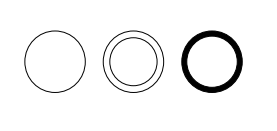
\includegraphics[width=\textwidth]{img/bpmn-event.png}
        \caption{Evento}
    \end{subfigure}
    \hfill
    \begin{subfigure}[b]{0.3\textwidth}
        \centering
        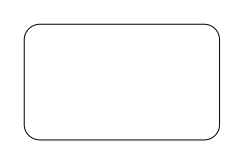
\includegraphics[width=\textwidth]{img/bpmn-activity.png}
        \caption{Actividad}
    \end{subfigure}
    \hfill
    \begin{subfigure}[b]{0.2\textwidth}
        \centering
        
\includegraphics[width=\textwidth]{img/bpmn-gateway.png}
        \caption{Pasarela}
    \end{subfigure}
    \caption{Elementos de flujo en diagramas BPMN}
    \label{fig:bpmn-elements}
\end{figure}

\subsection{Conectores}

Los elementos de flujo se conectan entre sí en un diagrama para crear la estructura básica de un proceso de negocio.
Hay tres conectores que proveen esta función.
Estos conectores son:

\begin{itemize}
    \item Flujos de secuencia
    \item Flujos de comunicación
    \item Asociaciones
\end{itemize}

\begin{figure}[H]
    \centering
    \begin{subfigure}[b]{0.3\textwidth}
        \centering
        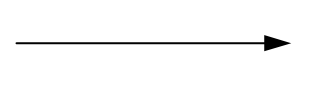
\includegraphics[width=\textwidth]{img/bpmn-sequence.png}
        \caption{Evento}
    \end{subfigure}
    \hfill
    \begin{subfigure}[b]{0.3\textwidth}
        \centering
        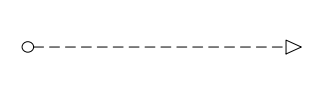
\includegraphics[width=\textwidth]{img/bpmn-message.png}
        \caption{Actividad}
    \end{subfigure}
    \hfill
    \begin{subfigure}[b]{0.3\textwidth}
        \centering
        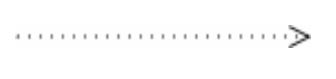
\includegraphics[width=\textwidth]{img/bpmn-association.png}
        \caption{Pasarela}
    \end{subfigure}
    \caption{Conectores en diagramas BPMN}
    \label{fig:bpmn-connectors}
\end{figure}

\subsection{Carriles}

Muchas metodologías de modelado de procesos utilizan el concepto de carriles como mecanismo para organizar las actividades en categorías visuales separadas con el fin de ilustrar diferentes capacidades funcionales o responsabilidades.
BPMN soporta los carriles con dos construcciones principales:

\begin{itemize}
    \item Pools
    \item Carriles
\end{itemize}

Los \textit{pools} se utilizan cuando el diagrama involucra dos entidades de negocio o participantes separados y están físicamente separados en el diagrama.
Las actividades dentro de pools separados se consideran procesos independientes. Por lo tanto, la secuencia no puede cruzar el límite de un pool.
Un flujo de mensaje se define como el mecanismo para mostrar la comunicación entre dos participantes, y, por lo tanto, debe conectarse entre dos pools.

Los \textit{carriles} están más estrechamente relacionados con las metodologías tradicionales de modelización de procesos por carriles de nado.
Los carriles se utilizan a menudo para separar las actividades asociadas a una función o rol específico de la empresa.
Una secuencia puede cruzar los límites de los carriles dentro de un pool, pero el flujo de mensajes no puede utilizarse entre los elementos de flujo de los carriles de un mismo grupo.

\begin{figure}[H]
    \centering
    \begin{subfigure}[b]{0.45\textwidth}
        \centering
        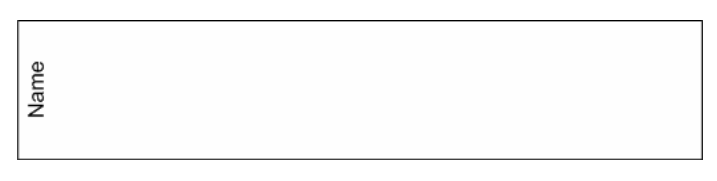
\includegraphics[width=\textwidth]{img/bpmn-pool.png}
        \caption{Pool}
    \end{subfigure}
    \hfill
    \begin{subfigure}[b]{0.45\textwidth}
        \centering
        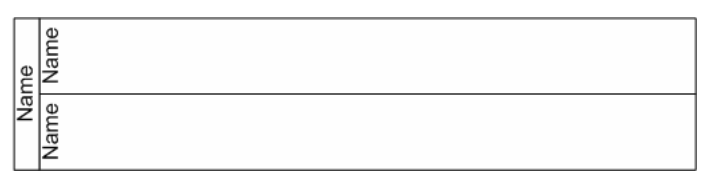
\includegraphics[width=\textwidth]{img/bpmn-lane.png}
        \caption{Carril}
    \end{subfigure}
    \caption{Carriles en diagramas BPMN}
    \label{fig:bpmn-pools}
\end{figure}

\subsection{Artefactos}

BPMN se diseñó para permitir a los modeladores y a las herramientas de modelado cierta flexibilidad a la hora de ampliar la notación básica y ofrecer la posibilidad de añadir el contexto adecuado a una situación de modelado específica.
Se puede añadir cualquier número de artefactos a un diagrama, según convenga para el contexto de los procesos de negocio que se están modelando.
La versión actual de la especificación BPMN predefine sólo tres tipos de artefactos, que son:

\begin{itemize}
    \item Documentos
    \item Agrupaciones
    \item Anotaciones
\end{itemize}

\begin{figure}[H]
    \centering
    \begin{subfigure}[b]{0.2\textwidth}
        \centering
        
\includegraphics[width=\textwidth]{img/bpmn-data.png}
        \caption{Documento}
    \end{subfigure}
    \hfill
    \begin{subfigure}[b]{0.3\textwidth}
        \centering
        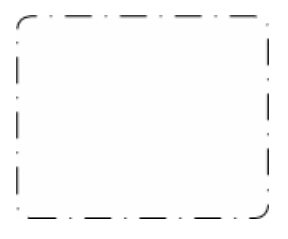
\includegraphics[width=\textwidth]{img/bpmn-group.png}
        \caption{Agrupación}
    \end{subfigure}
    \hfill
    \begin{subfigure}[b]{0.4\textwidth}
        \centering
        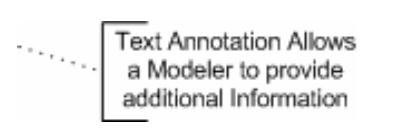
\includegraphics[width=\textwidth]{img/bpmn-note.png}
        \caption{Anotación}
    \end{subfigure}
    \caption{Artefactos en diagramas BPMN}
    \label{fig:bpmn-artifacts}
\end{figure}


\section{Análisis de la causa raíz. Cinco porqués}

El método de los cinco porqués para el análisis de la causa raíz fue desarrollado por Sakichi Toyota como parte del Sistema de Producción Toyota.
Ha sido ampliamente adoptado tanto en programas Lean como Six Sigma \cite{tarantino_smart_2022}.
A primera vista, el método de los cinco porqués parece una técnica simplista con un valor limitado, pero es eficaz y fácil de utilizar para llegar a las causas profundas de los problemas menos complejos.
Funciona porque elimina los síntomas de un problema, capa por capa, hasta llegar al "por qué" final, que es la raíz.

\subsection{Proceso}

El ejercicio de los cinco porqués mejora enormemente cuando lo aplica un equipo y hay cinco pasos básicos para llevarlo a cabo. En la Figura~\ref{fig:five-whys} se muestra una plantilla a modo de ejemplo.

\begin{itemize}
    \item Reunir a un equipo y desarrollar el planteamiento del problema de común acuerdo. Una vez hecho esto, se decide si se necesitan más personas para resolver el problema.
    \item Se pregunta el primer "por qué" al equipo: ¿por qué se produce tal o cual problema? Probablemente habrá tres o cuatro respuestas sensatas: se anotan todas en un folio o pizarra, o con fichas pegadas a la pared.
    \item Se preguntan otros cuatro "por qué" sucesivos, repitiendo el proceso para cada afirmación en el folio, la pizarra o las fichas. Coloque cada respuesta cerca de su "padre". Se realiza un seguimiento de todas las respuestas plausibles. Cuando la pregunta "¿por qué?" no aporte más información útil, se habrá identificado la causa principal. (Si es necesario, se siguen haciendo preguntas más allá de las cinco capas arbitrarias para llegar a la causa raíz).
    \item Entre la docena de respuestas a la última pregunta "¿por qué?", se buscan las causas sistémicas del problema. Se discuten con el fin de decidir la causa sistémica más probable. Después de la sesión en equipo, es recomendable un \textit{debriefing} y mostrar el producto a los demás para confirmar que ven la lógica en el análisis.
    \item Tras determinar la causa raíz más probable del problema y obtener confirmación de la lógica que subyace al análisis, se desarrollan las medidas correctivas adecuadas para eliminar la causa raíz del sistema. Las acciones pueden ser emprendidas por otros, pero la planificación y ejecución se beneficiarán de las aportaciones del equipo.
\end{itemize}

\begin{figure}
    \centering
    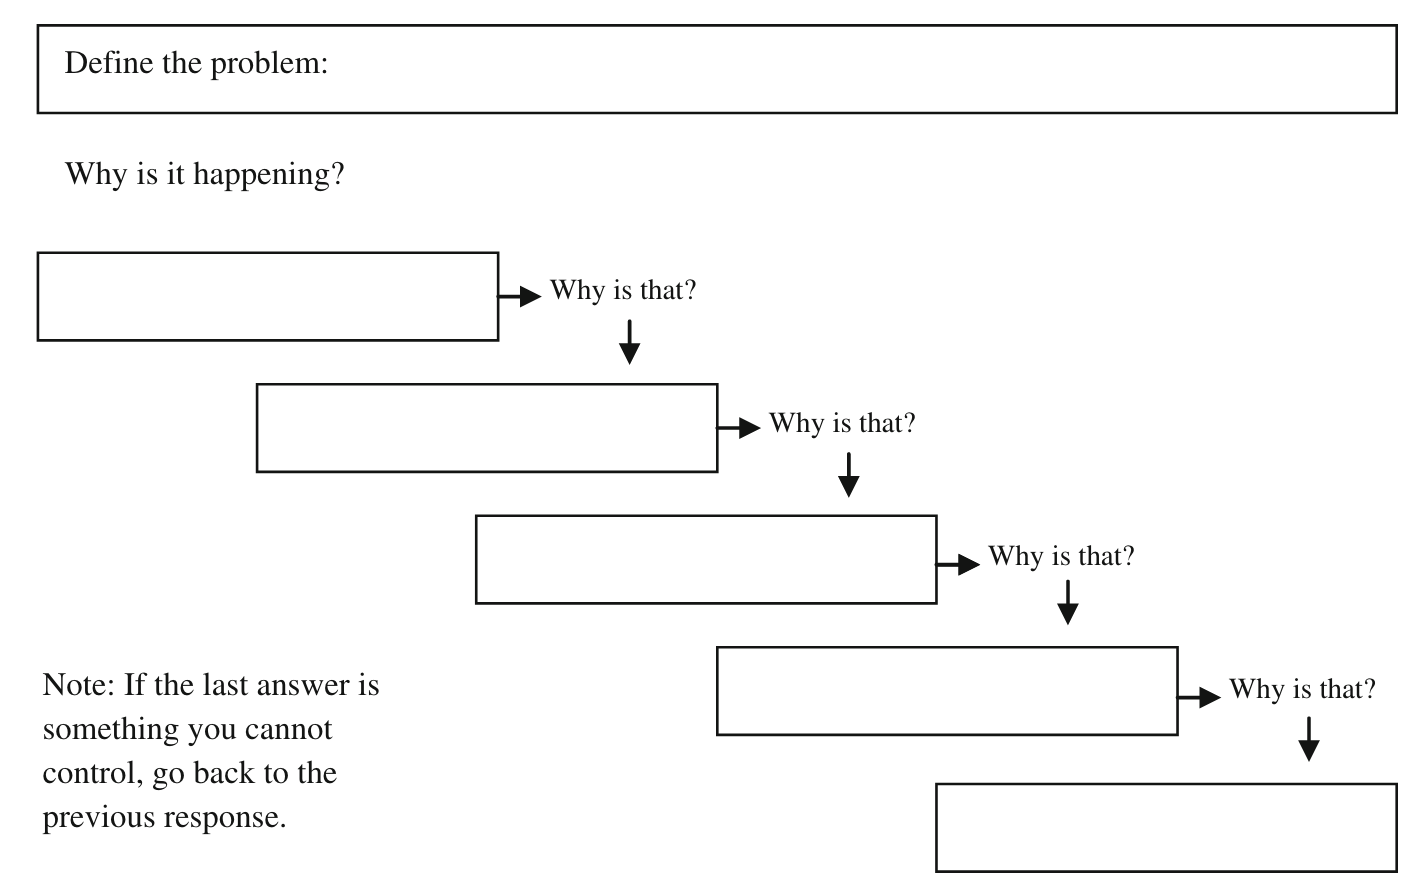
\includegraphics[width=0.8\textwidth]{img/five-whys.png}
    \caption{Plantilla de ejemplo de los cinco porqués. Fuente: \citetitle{serrat_five_2017}}
    \label{fig:five-whys}
\end{figure}

\subsection{Precauciones}

La técnica de los cinco porqués ha sido criticada por ser una herramienta demasiado básica para analizar las causas raíz con la profundidad necesaria para garantizar que las causas se solucionan.
Entre las razones de esta crítica se incluyen:

\begin{itemize}
    \item La tendencia de los investigadores a detenerse en los síntomas y no proceder a las causas profundas de nivel inferior.
    \item La incapacidad de los investigadores para ir más allá de la información y los conocimientos actuales.
    \item Falta de facilitación y apoyo para ayudar a los investigadores a formular las preguntas adecuadas.
    \item La baja tasa de repetición de los resultados: se sabe que diferentes equipos que utilizan la técnica de los cinco porqués llegan a diferentes causas para el mismo problema.
\end{itemize}

Es evidente que la técnica de los cinco porqués se resentirá si se aplica únicamente por deducción \cite{serrat_five_2017}.
El proceso articulado anteriormente fomenta la verificación sobre el terreno de las respuestas a la pregunta "por qué" actual antes de pasar a la siguiente, y debería ayudar a evitar estos problemas.